Os resultados alcançados pelo trabalho em estudo dizem respeito a três fases do desenvolvimento que se resumem em: 
\begin{itemize}
	\item Coleta de dados dos pacientes;
	\item Produção do \textit{software} GPSATWeb;
	\item Desenvolvimento da RNA.
\end{itemize}

\section{Coletas de dados}
	Um dos três pilares deste trabalho, a coleta de dados com os pacientes, foi o processo mais longo do desenvolvimento do trabalho. Isso pois, eram necessários voluntários que se dispusessem a participar, e, a deixar-se ser examinado pela profissional de saúde que liderou esta fase. Outro problema encontrado foi a dificuldade de locomoção dos pacientes até o laboratório onde foi produzida a pesquisa, necessitando-se até mesmo que os pesquisadores fossem, algumas vezes, até suas residências para que pudesse acontecer a coleta.

	O modelo de coleta proposto foi aplicado em 13 pacientes, dentro e fora do laboratório, sempre seguindo a estrutura da ficha proposta (Anexo A). Todos os pacientes avaliados assinaram um Termo de Consentimento Livre e Esclarecido (TCLE, Anexo B) para que as avaliações de seu coto pudessem ser feitas. Após a avaliação feita pela profissional de saúde, era aplicada a sessão de fotos do coto do paciente para posterior análise. Nas primeiras coletas, as fotos tiradas focavam o coto do paciente de um ângulo externo, como mostra a Figura 13.

	\begin{figure}[ht]
	    \centering
	    \label{fig13}
	        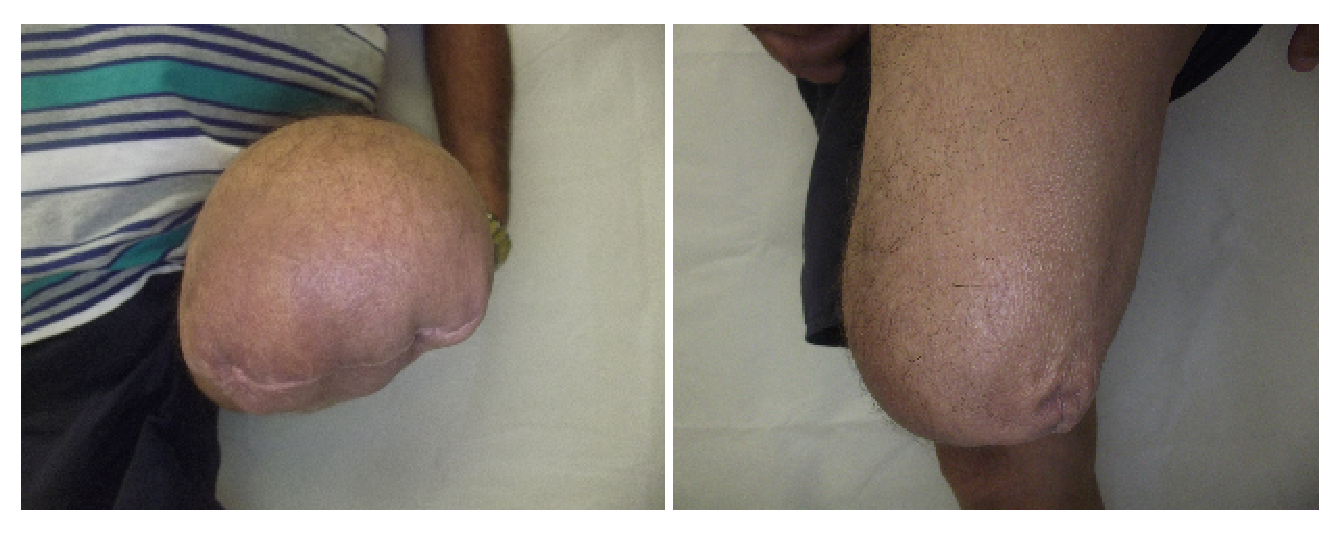
\includegraphics[keepaspectratio=true, scale=0.6]{editaveis/images/figura_coto.eps}
	    \caption{Fotos do coto de um paciente tiradas em laboratório.}
	\end{figure} 

	Entretanto, com as fotos tiradas neste tipo de posicionamento, seria necessário um tratamento de imagem para que pudessem ser enviadas posteriormente para treinamento da RNA. Então, neste momento, o ângulo de visão das fotos foi alterado para que todos os \textit{pixels} da imagem possuíssem somente informação da pele do coto do paciente, como pode ser visto na Figura 14.

	\begin{figure}[ht]
	    \centering
	    \label{fig14}
	        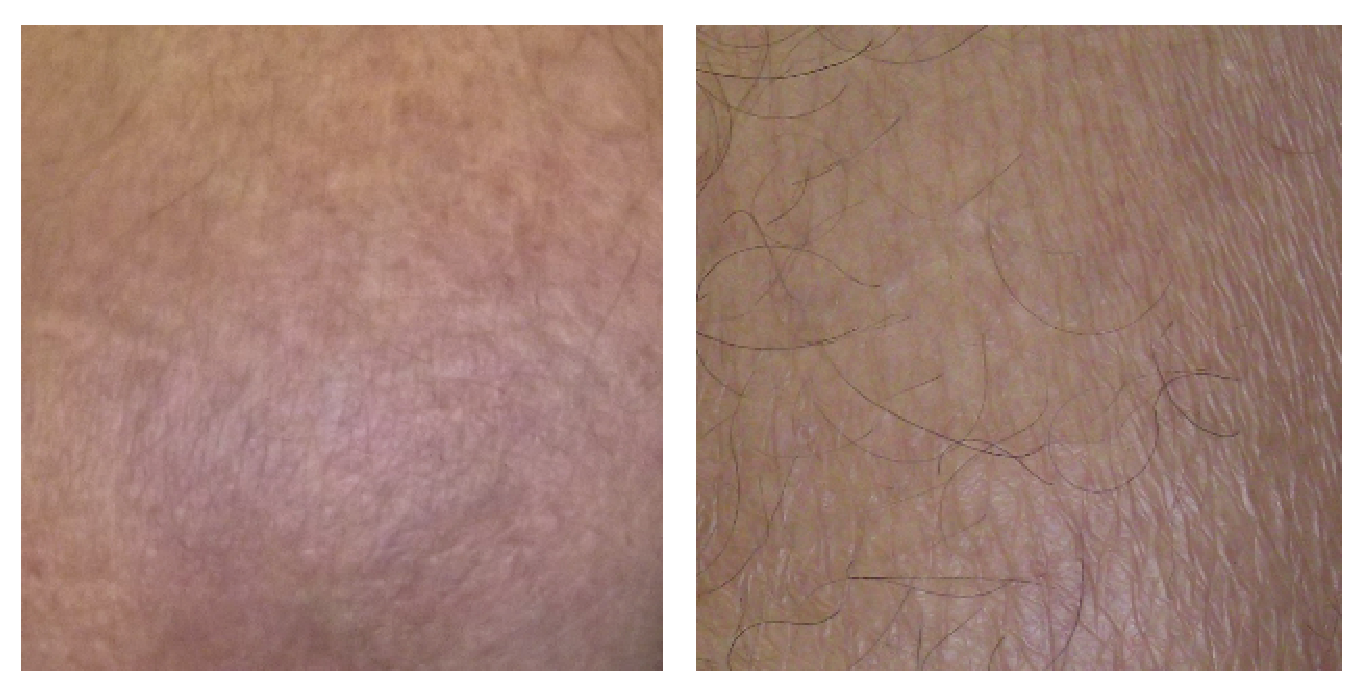
\includegraphics[keepaspectratio=true, scale=0.6]{editaveis/images/figura_coto_corte.eps}
	    \caption{Fotos focadas na pele do coto do paciente tiradas em laboratório.}
	\end{figure} 


\section{Desenvolvimento do GPSATWeb}
	O desenvolvimento do \textit{software} pode ser dividido em duas fases, o desenvolvimento do sistema \textit{web} e o desenvolvimento da \textit{api}. 

	O sistema \textit{web} foi produzido em duas fases temporais destintas. Na primeira, o objetivo era construir o sistema \textit{web} utilizando uma tecnologia nova na área de produção de interfaces para a \textit{web} chamada ReactJS. O ReactJS é uma biblioteca JavaScript de código aberto mantida pelo Facebook, e pela comunidade de \textit{software} livre, que visa facilitar e agilizar o processo de construção de interfaces de usuário. Por ser uma tecnologia recente, durante esta primeira fase de produção, a curva de aprendizagem desta tecnologia atrapalhou o ritmo de desenvolvimento do sistema, fazendo que sua entrega fosse atrasada.

	Na segunda fase temporal, tudo o que foi produzido aplicando-se o ReactJS foi retirado do projeto, e, o mesmo substituído pelo \textit{framework} Django, utilizando-se a linguagem de programação \textit{Python}. A partir deste momento, a produção do sistema começou a fluir num ritmo mais acelerado e o \textit{software web} foi finalizado como mostra a Figura 15.
	\newpage
	\begin{figure}[ht]
	    \centering
	    \label{fig15}
	        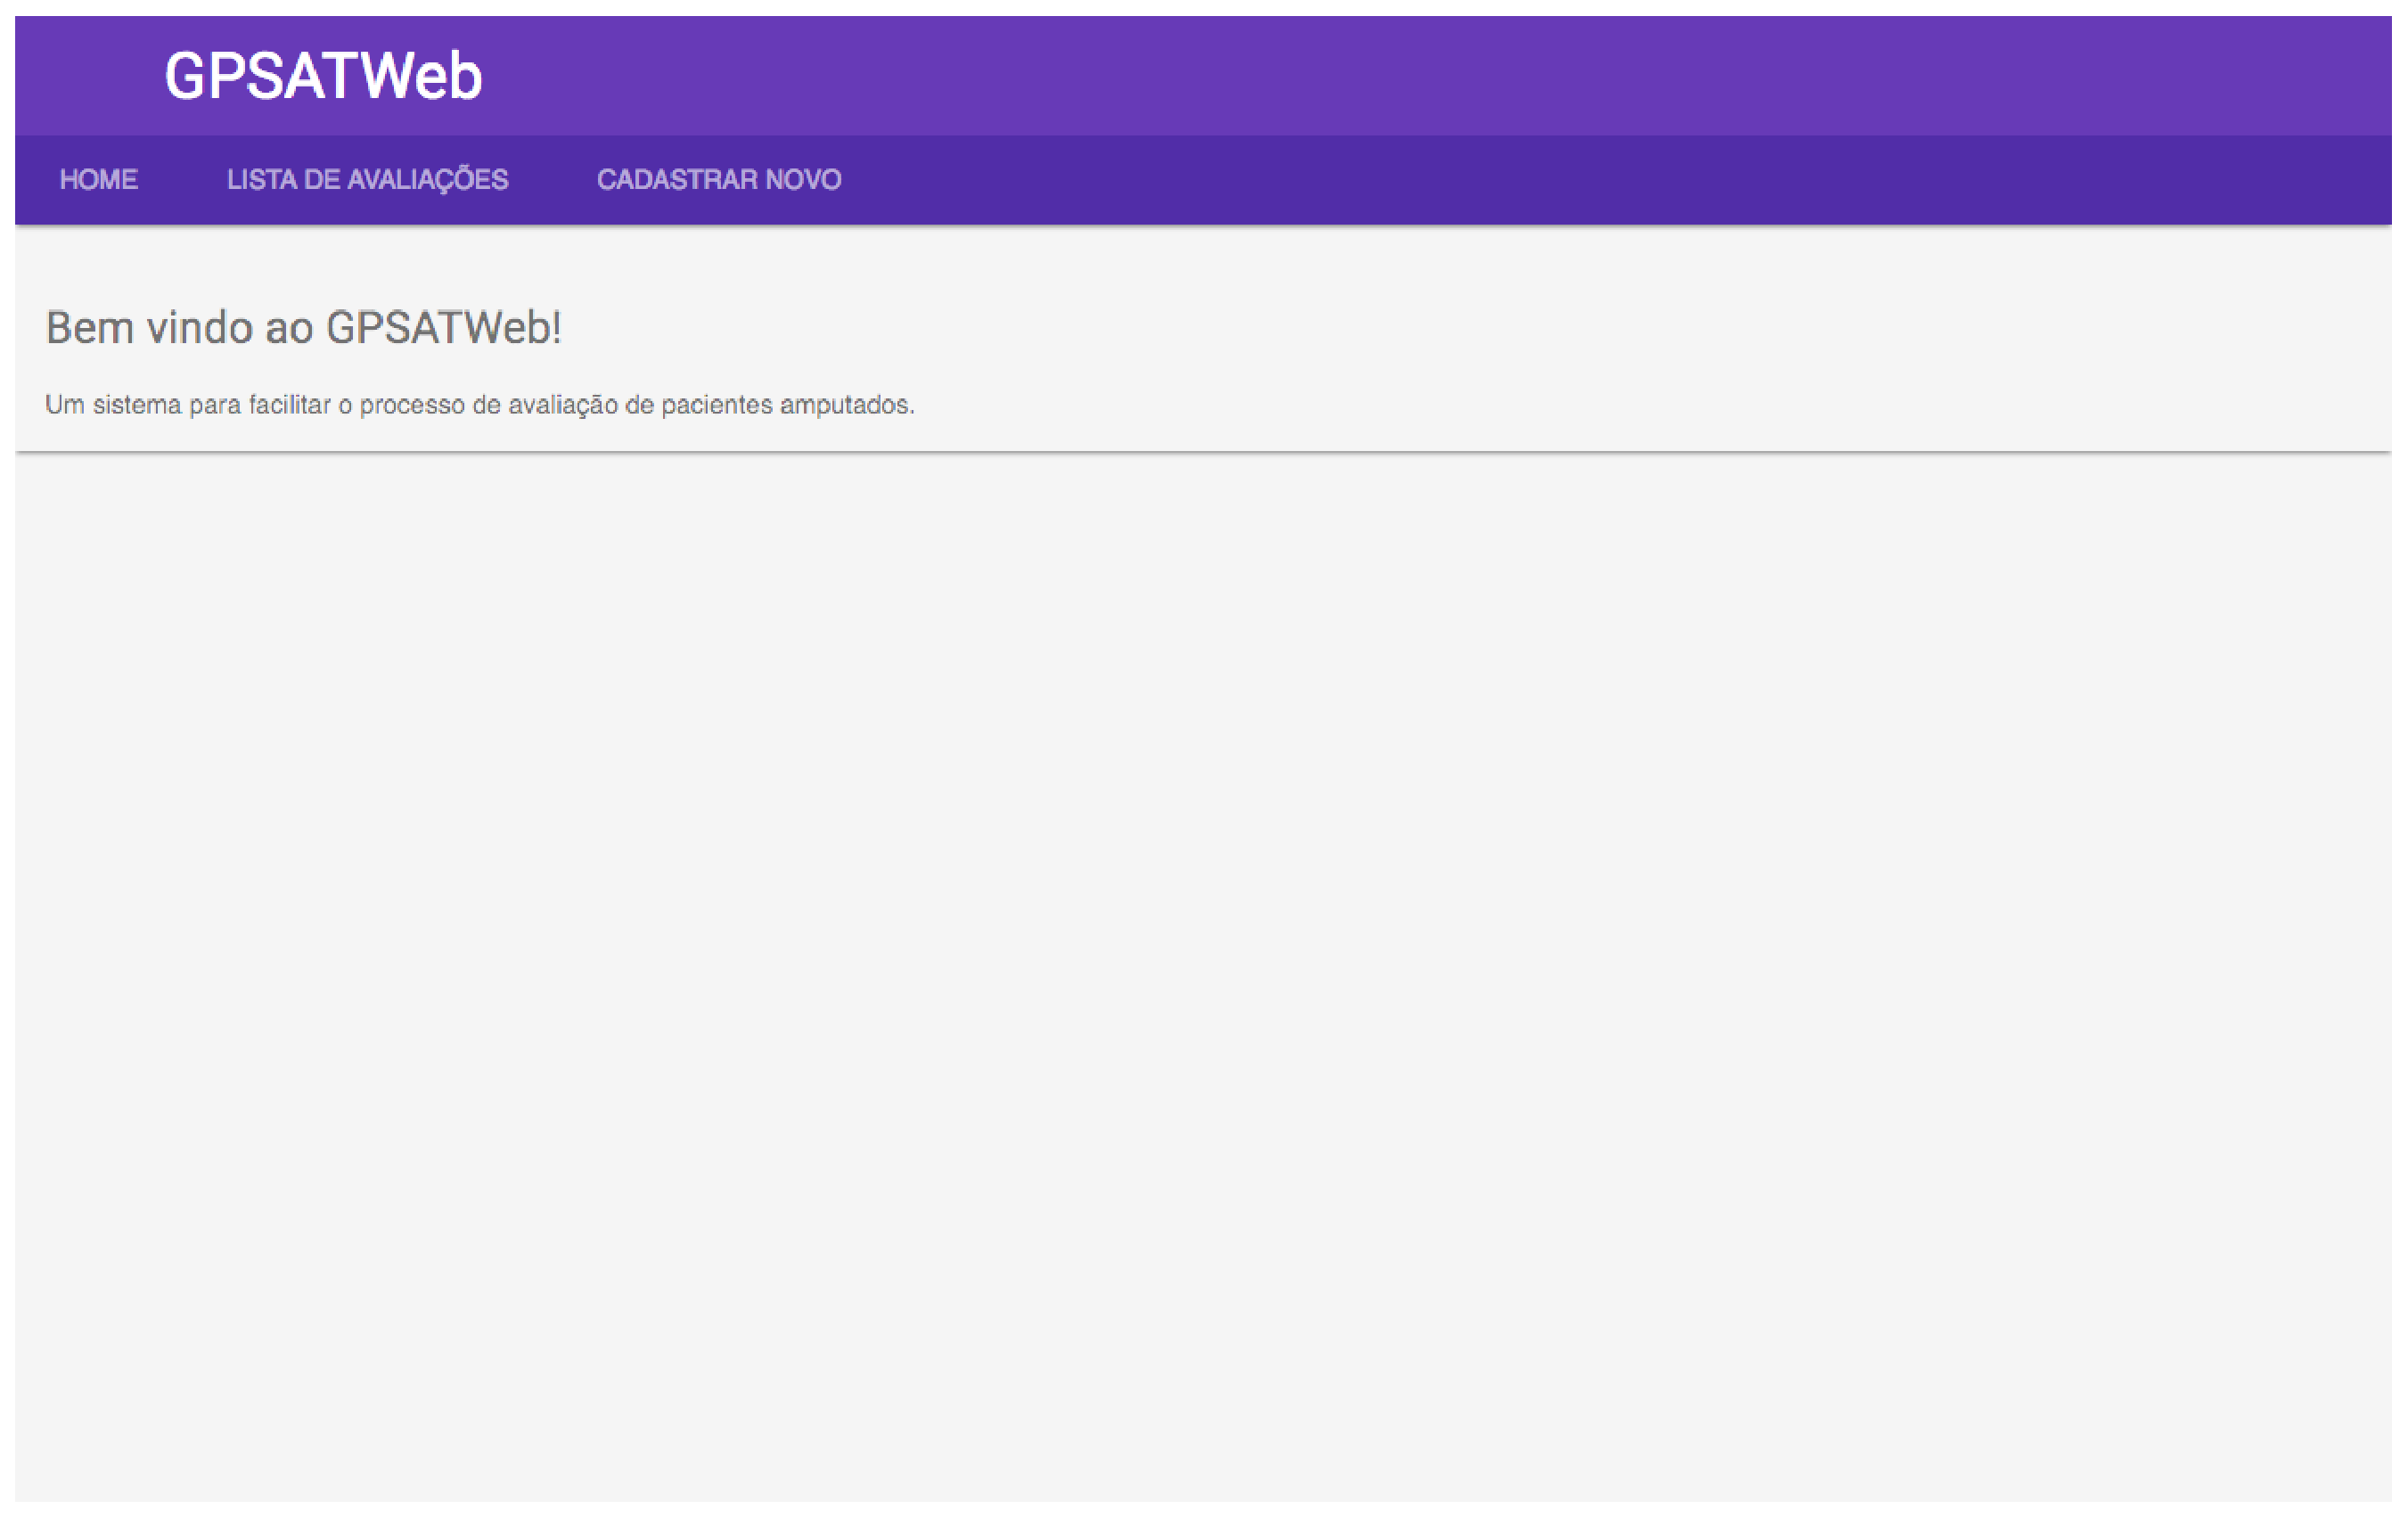
\includegraphics[keepaspectratio=true, scale=0.23]{editaveis/images/tela_inicial.eps}
	    \caption{Tela inicial do GPSATWeb.}
	\end{figure} 

	O GPSATWeb tem uma aparência simples, produzida para facilitar a usabilidade do sistema por qualquer pessoa. Existem apenas duas abas de ação no menu:

	\begin{itemize}
		\item Lista de Avaliações: onde se encontra uma lista com todas as avaliações já efetuadas utilizando-se o sistema, com um botão que permite ver todas as informações de uma determinada avaliação em uma nova tela, como mostra a Figura 16, e, acaso ainda não haja nenhuma avaliação salva, simplesmente mostra uma mensagem de que não foi feita nenhuma avaliação;

		\begin{figure}[ht]
		    \centering
		    \label{fig16}
		        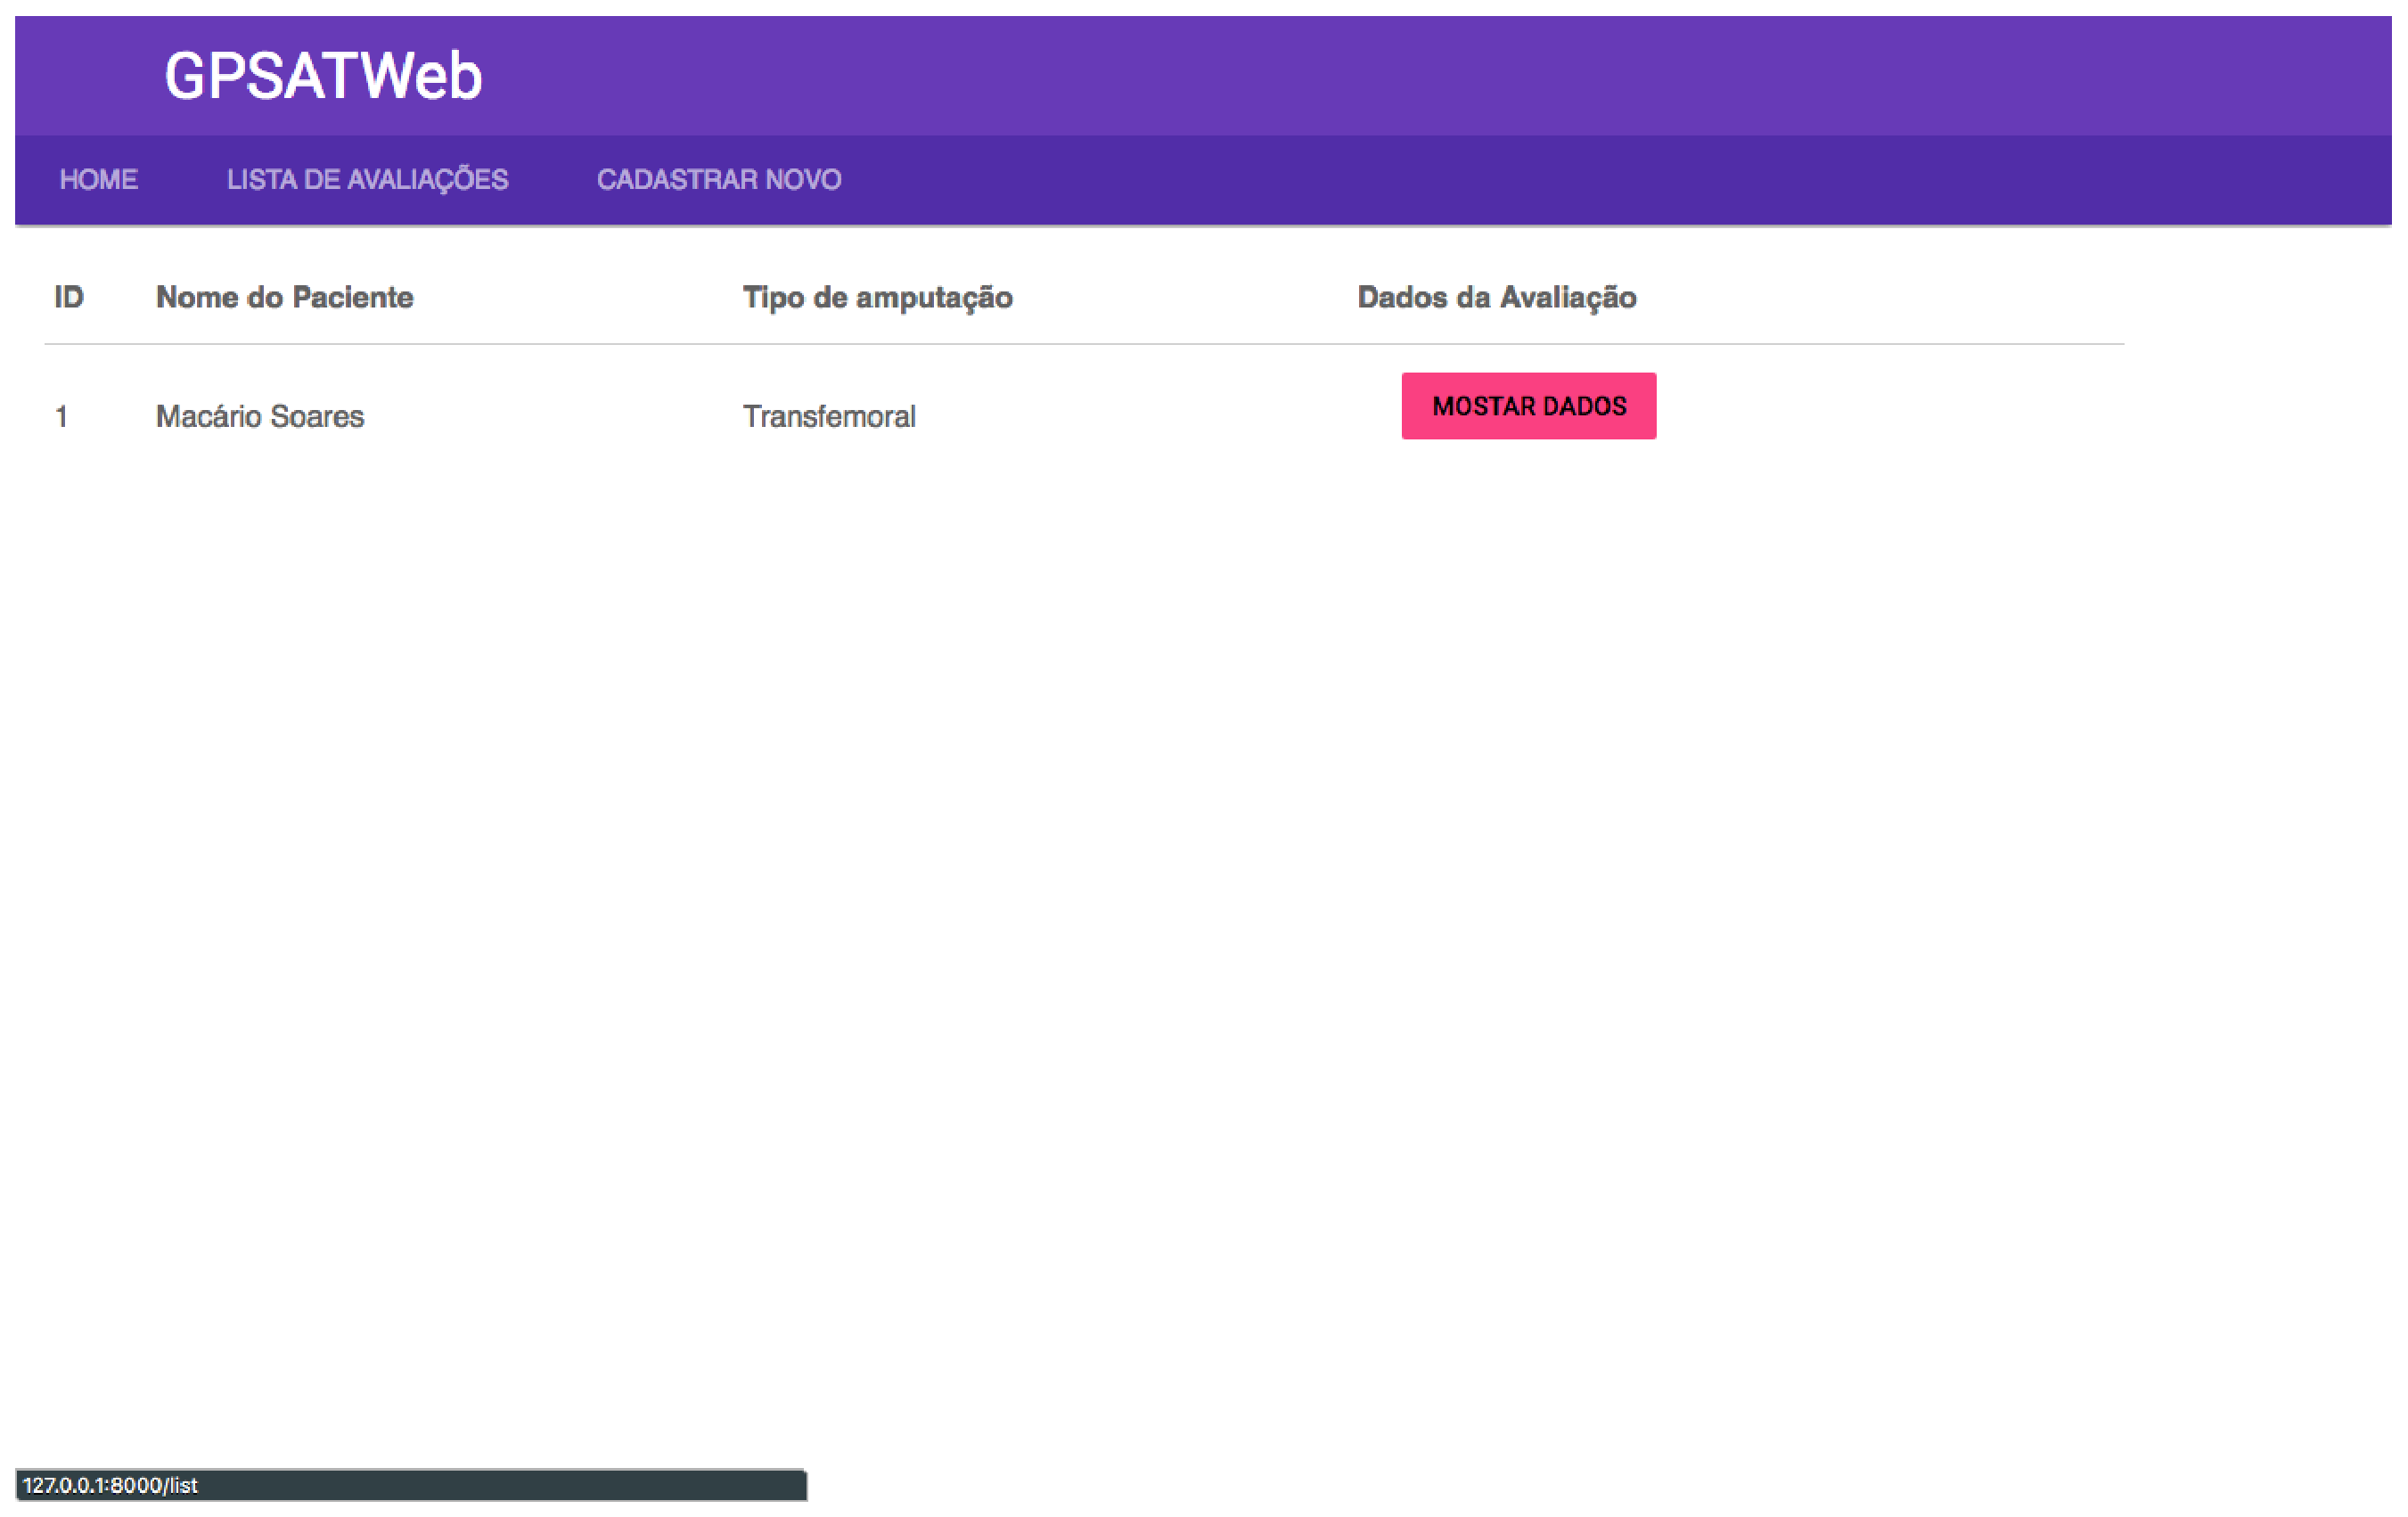
\includegraphics[keepaspectratio=true, scale=0.23]{editaveis/images/tela_lista.eps}
		    \caption{Tela da listagem de avaliações cadastradas.}
		    (Paciente fictício cadastrado a título de demonstração)
		\end{figure} 


		\item Cadastrar Novo: onde se sencontra a ficha de avaliação do paciente (Anexo I) para ser preenchida enquanto o profissional da saúde avalia o paciente no laboratório (ou consultório), mostrado na Figura 17.
	\end{itemize}

	\begin{figure}[ht]
	    \centering
	    \label{fig17}
	        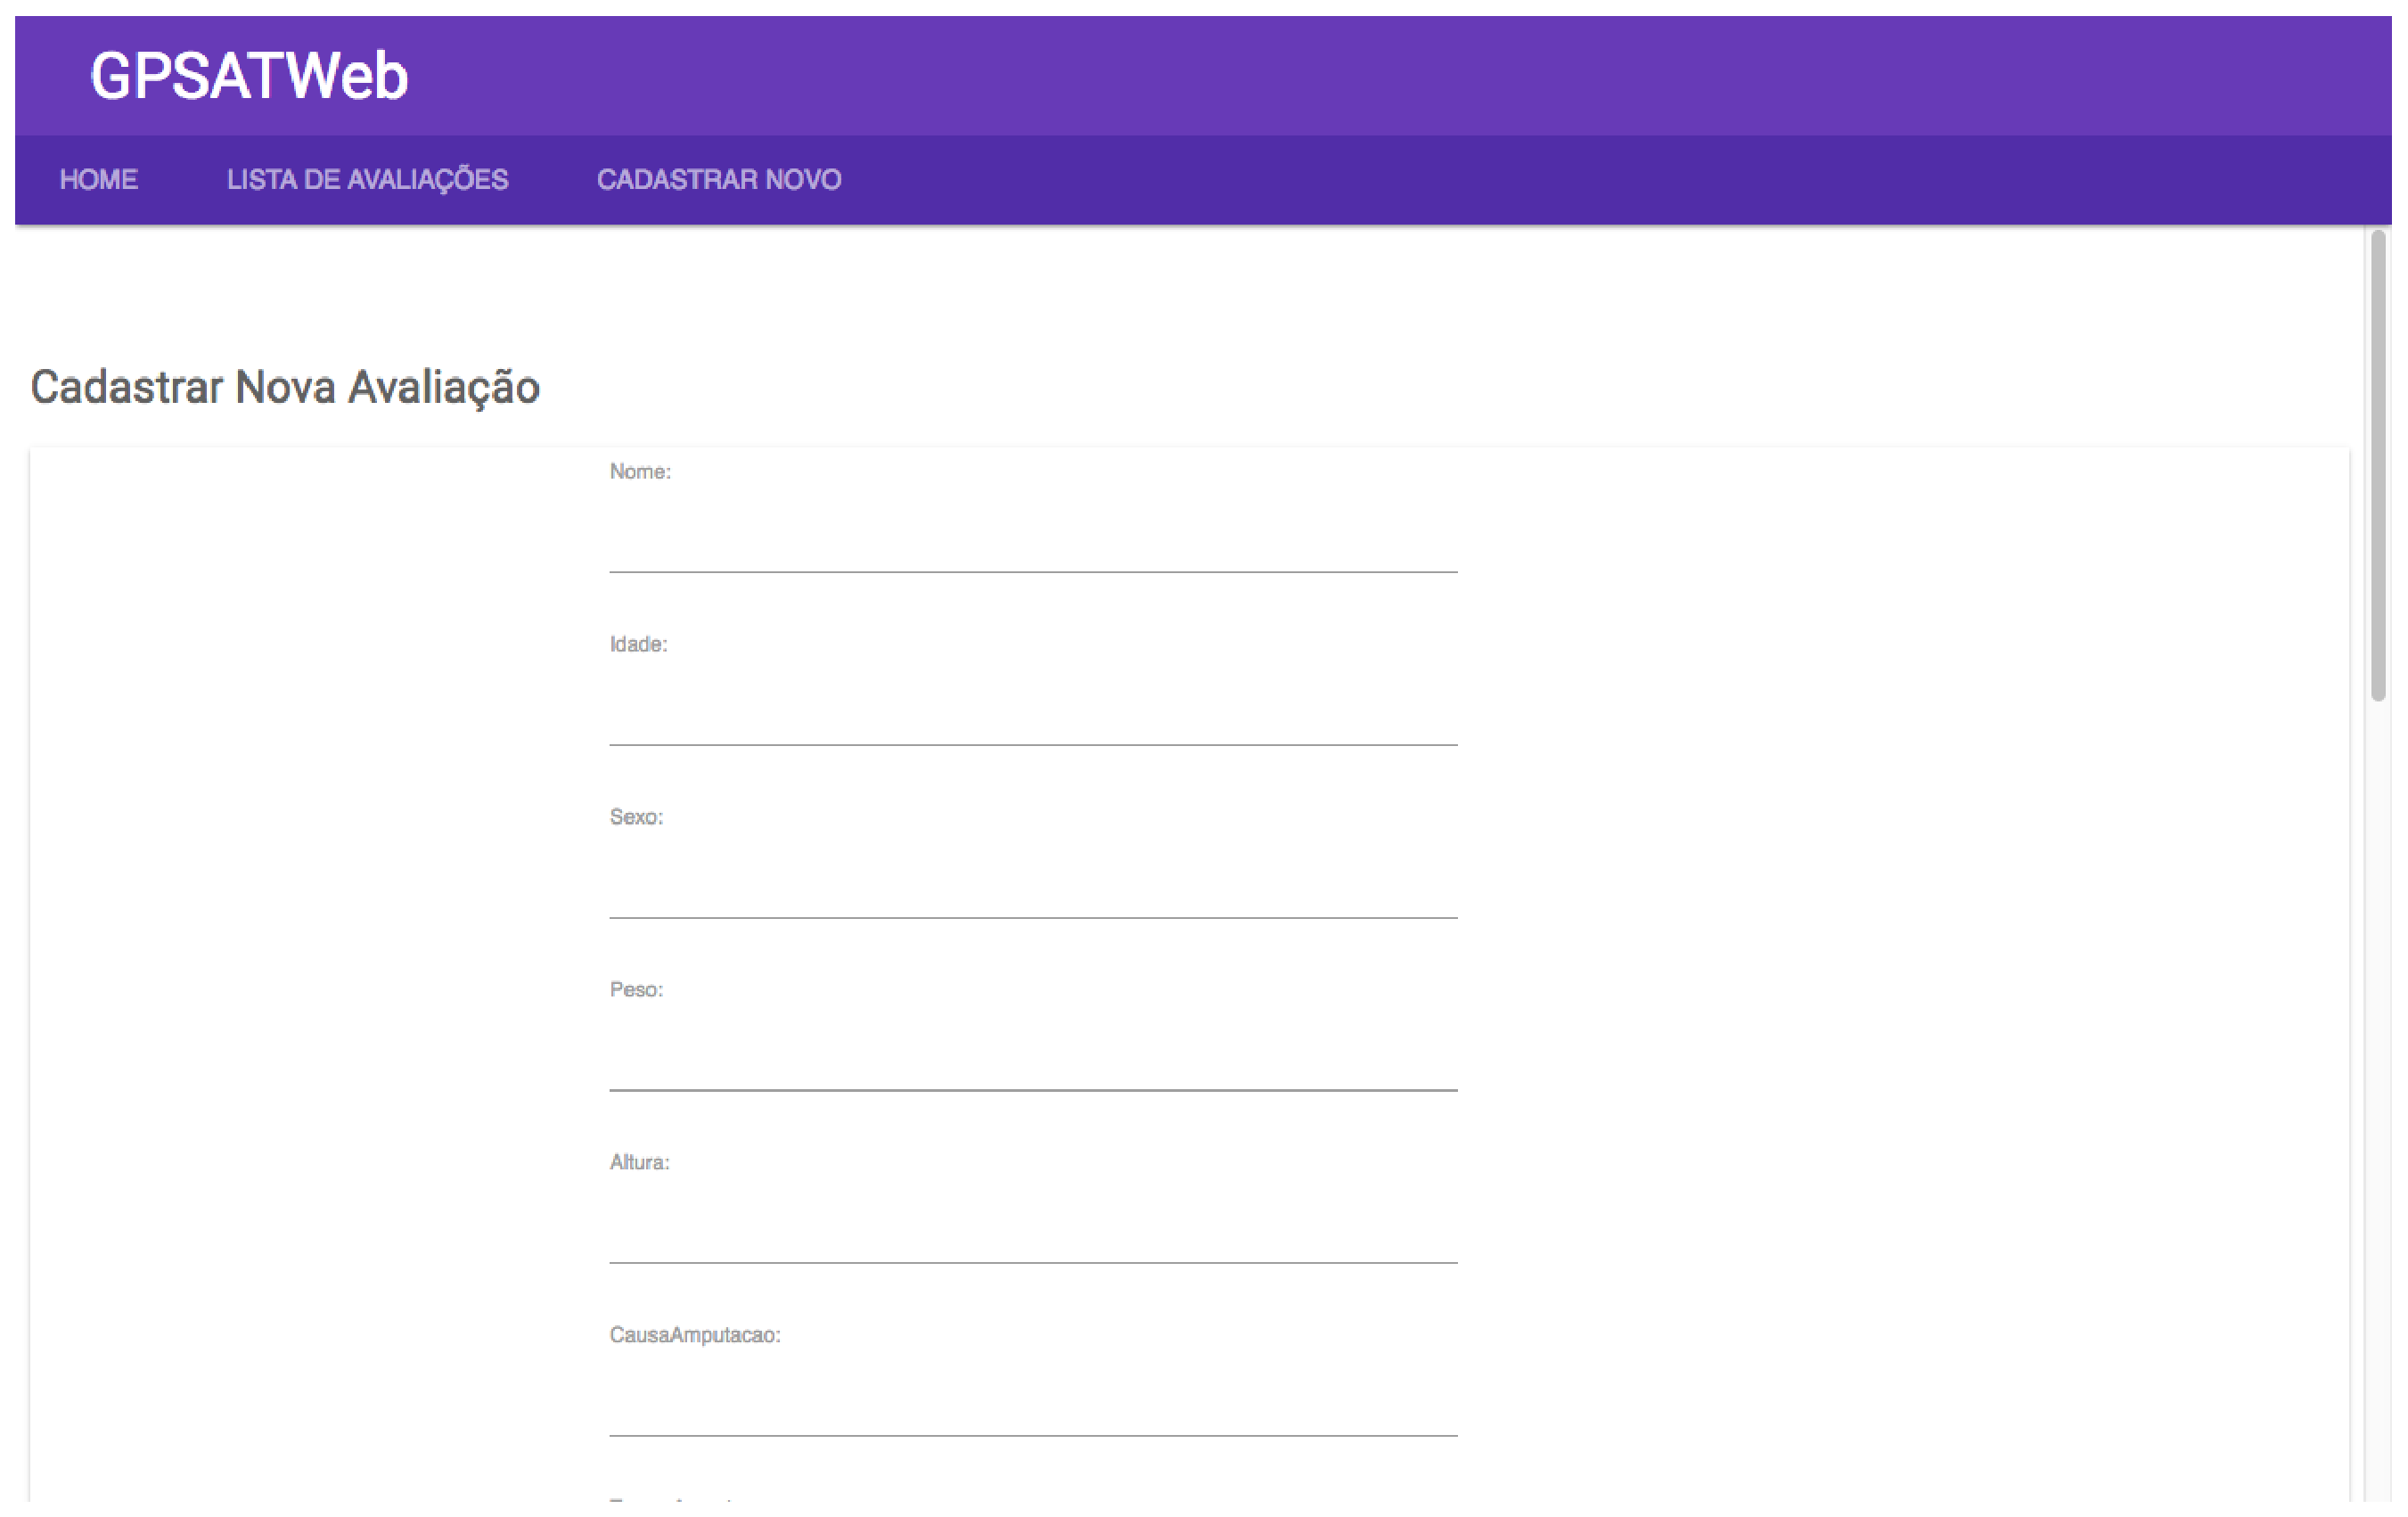
\includegraphics[keepaspectratio=true, scale=0.23]{editaveis/images/tela_cadastro.eps}
	    \caption{Tela da listagem de avaliações cadastradas.}
	    (Paciente fictício cadastrado a título de demonstração)
	\end{figure} 

	A \textit{API Restful} foi construída também utilizando o \textit{framework} Django em linguagem de programação \textit{Python}. Foi construída paralelamente ao sistema \textit{web}, sendo seu serviço de dados. Neste momento, existem dois fluxos básicos de interação do sistema \textit{web} com a \textit{api}. O primeiro é o de cadastro de uma nova avaliação, como mostra a Figura 18.

	\begin{figure}[ht]
	    \centering
	    \label{fig18}
	        \includegraphics[keepaspectratio=true, scale=0.55]{editaveis/images/sequencia_cadastrar.eps}
	    \caption{Diagrama de sequência de cadastro de nova avaliação.}
	\end{figure} 

	O segundo fluxo básico de interação entre o sistema \textit{web} com a \textit{api} é o de listagem de todas as avaliações já feitas em uma página e, posteriormente de mostrar o conteúdo de uma avaliação específica selecionada pelo usuário, como mostrado na Figura 19.

	\begin{figure}[ht]
	    \centering
	    \label{fig19}
	        \includegraphics[keepaspectratio=true, scale=0.55]{editaveis/images/sequencia_listar.eps}
	    \caption{Diagrama de sequência de listagem de avaliações.}
	\end{figure} 


\section{Rede Neural Artificial}

	A RNA MLP proposta neste trabalho foi construída utilizando-se a biblioteca \textit{python} Scikit Learn e treinada utilizando o algorítmo \textit{Backpropagation}. A RNA está estruturada em três camadas:

	\begin{itemize}
		\item Camada de entrada: composta por 1024 neurônios, um para cada \textit{pixel} da imagem de entrada no sistema que tem tamanho de 32x32 \textit{pixels};
		\item Camada intermediária: composta por 34 neurônios, calculados utilizando-se a equação \textit{NI} = \textit{NS} + $\sqrt{\textit{NE}}$ proposta por \cite{Eberhart1991}, onde NI é a quantidade de neurônios na camada intermediária, NS é a quantidade de neurônios na camada de saída e NE a quantidade de neurônios na camada de entrada;
		\item Camada de saída: composta de 3 neurônios de saída, os quais classificam individualmente a condição da pele do paciente entre três possíveis saídas: normal, pálido ou cianótico.
	\end{itemize}

	Os parâmetros da RNA MLP, tais como a função de ativação, taxa de aprendizado, \textit{momentum}, quantidade máxima de iterações, entre outros, foram definidos utilizando-se dos valores e \textit{ranges} aceitos pelo classificador \textit{MLPClassifier} persente na biblioteca Scikit Learn. Além disso, os valores dos parâmetros de entrada da RNA foram descritos em código manualmente, sendo variados de a cordo com o desempenho apresentado pela RNA no processo experimental. Os valores padrões fornecidos pela ferramenta, são intervalos tipicamente encontrados na literatura para resolver em problemas básicos de ML. O trecho de código a seguir mostra um classificador MLP padrão da biblioteca Scikit Learn.

	\begin{lstlisting}
		MLPClassifier(hidden_layer_sizes=(100, ), activation='relu', solver='adam', alpha=0.0001, batch_size='auto', learning_rate='constant', learning_rate_init=0.001, power_t=0.5, max_iter=200, shuffle=True, random_state=None, tol=0.0001, verbose=False, warm_start=False, momentum=0.9, nesterovs_momentum=True, early_stopping=False, validation_fraction=0.1, beta_1=0.9, beta_2=0.999, epsilon=1e-08)
	\end{lstlisting} 

	Durante o procedimento experimental da RNA, a cada experimento realizado para medir a taxa de acerto do classificador, um dos valores foram variados, até que se obteve a melhor taxa de acerto da RNA até então. Por conta deste processo experimental, os valores obtidos não necessariamente são os melhores para um outro tipo de problema, visto que, as variações dos parâmetros foram feitas a fim de conseguir um melhor resultado para esta RNA. Sendo assim, os valores que estão sendo utilizados na RNA MLP produzida neste trabalho são mostrados no código a seguir.

	\begin{lstlisting}
		MLPClassifier(hidden_layer_sizes=(34 ), activation='tanh', solver='adam', alpha=0.001, momentum=0.9, nesterovs_momentum=True, batch_size='auto', max_iter=500, early_stopping=False, random_state=None, tol=0.0001, learning_rate='constant', learning_rate_init=0.0001, power_t=0.3, verbose=True, warm_start=True, validation_fraction=0.1, beta_1=0.9, beta_2=0.999, epsilon=1e-08)
	\end{lstlisting} 

	Seguindo estes parâmetros, a Figura 20 mostra o treinamento da RNA MLP para o problema proposto de classificação dos tipos de pele dos cotos dos pacientes.

	\begin{figure}[ht]
	    \centering
	    \label{fig20}
	        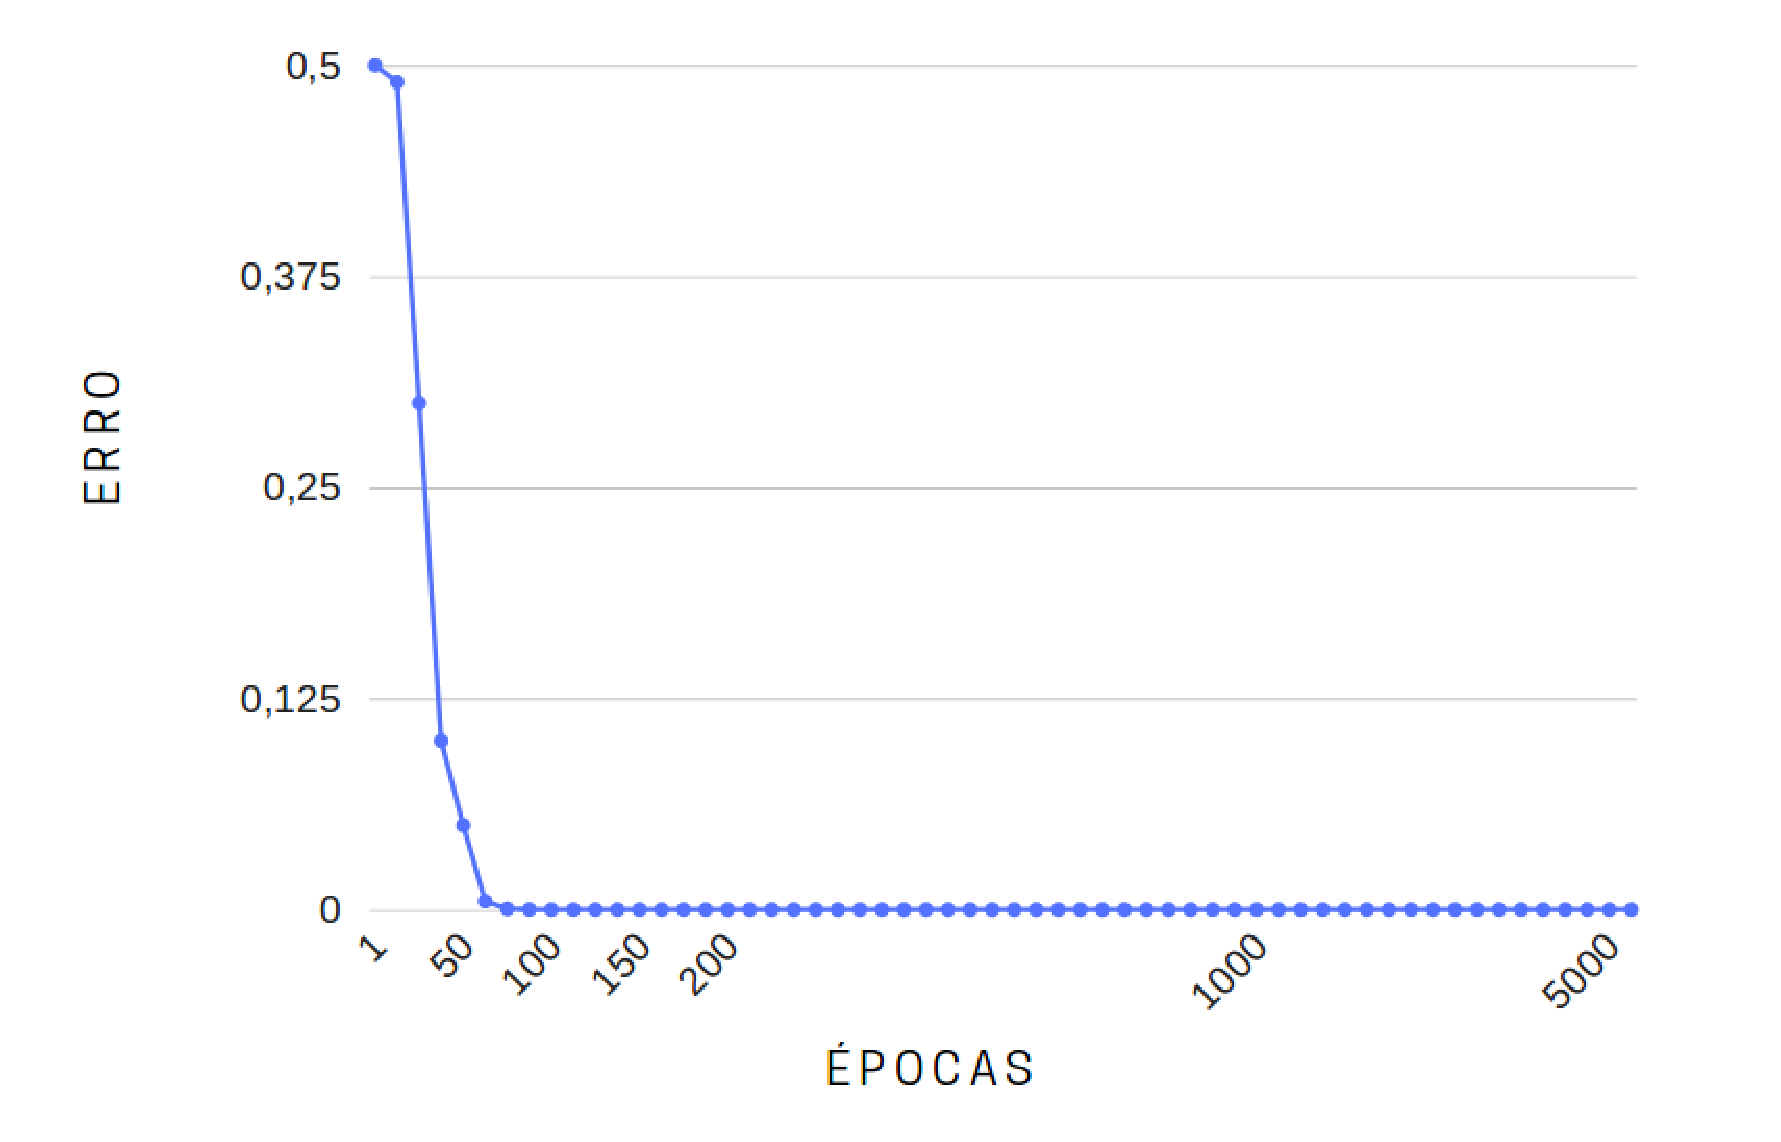
\includegraphics[keepaspectratio=true, scale=0.5]{editaveis/images/grafico_rna.eps}
	    \caption{Gráfico de treinamento da RNA MLP.}
	\end{figure} 


	\subsection{Teste e Validação}

		Na fase de coleta de dados com os pacientes foram feitas 3 fotografias de cada paciente mostrando ângulos diferentes e evidenciando a pele do coto. Depois disso, cada foto foi cortada em 5 quadrados de 32x32 \textit{pixels}, os quais apresentavam em seus \textit{pixels} apenas informação de pele do paciente. Ao fim desta fase, visto que foram feitas coletas de dados com 13 pacientes, a massa de dados de imagens de entrada para a RNA é de 195 imagens. Tais imagens foram divididas em dois grupos, o primeiro com as imagens que foram designadas para treinamento da RNA e o segunso com as imagens designadas para a fase de teste da RNA. 

		Foram feitos três testes diferentes para medir a acurácia da RNA MLP de acordo com a quantidade de fotos usadas para treinamento e teste:
		\begin{itemize}
			\item Teste 1: 75\% das fotos (146 imagens) foram designadas para a massa de treinamento da RNA, enquanto os outros 20\% (48 imagens) foram disponibilizadas para a fase de teste da RNA. 
			\item Teste 2: 80\% das fotos (156 imagens) foram designadas para a massa de treinamento da RNA, enquanto os outros 20\% (39 imagens) foram disponibilizadas para a fase de teste da RNA. 
			\item Teste 3: 85\% das fotos (166 imagens) foram designadas para a massa de treinamento da RNA, enquanto os outros 20\% (29 imagens) foram disponibilizadas para a fase de teste da RNA. 
		\end{itemize}

		O valor da taxa de acerto da RNA construída, de acordo com os parâmetros citados, pode ser observada na Tabela 2. 

		\begin{table}[H]
			\centering
			\caption{Taxa de acerto da RNA.}
			\label{tab02}
			\begin{tabular}{|l|l|}
				\hline
				Porcentagem da massa de dados usada para teste & Taxa de acerto da RNA \\ \hline
				25\%                                           & 77.54\%               \\ \hline
				20\%                                           & 77.27\%               \\ \hline
				15\%                                           & 77.25\%               \\ \hline
			\end{tabular}
			
		\end{table}

		Como é observado na Tabela 2, as taxas de acerto da RNA MLP foram muito próximas entre si. Isso acontece pois a massa de dados usada para treinamento e testes ainda é muito restrita. A baixa quantidade de pacientes e consequentimente de tipos de pele dos cotos que tiveram dados coletados, causam esta baixa variação de acerto da RNA MLP. Sendo assim o ideal seria que houvessem mais amostras para que o modelo de RNA MLP construído pudesse evoluir ainda mais. 

% Os resultados alcançados no projeto se dividiram em duas fases diferentes: o \textit{software} GPSATWeb, desenvolvido para aplicação da ficha de avaliação dos amputados; a RNA, que apresenta uma análise da condição de pele dos amputados com a utilização de fotos como dados de entrada.

% O \textit{software web} foi finalizado e é funcional. Este sistema visa facilitar e agilizar a aplicação e o preenchimento da ficha de avaliação dos pacientes amputados, além de salvar seguramente seus dados e gerar um relatório da avaliação contendo o histórico do paciente.

% A RNA trabalhada foi construída em um processo iterativo de variação de entrada para que sua precisão fosse gradualmente aumentada a cada iteração. No início do processo foi construída também uma RNA utilizando outro método de treinamento para avaliar, a título de comparação, o crescimento da precisão da RNA MLP, como pode ser visto na Figura 9.

% \begin{figure}[ht]
%     \centering
%     \label{fig09}
%         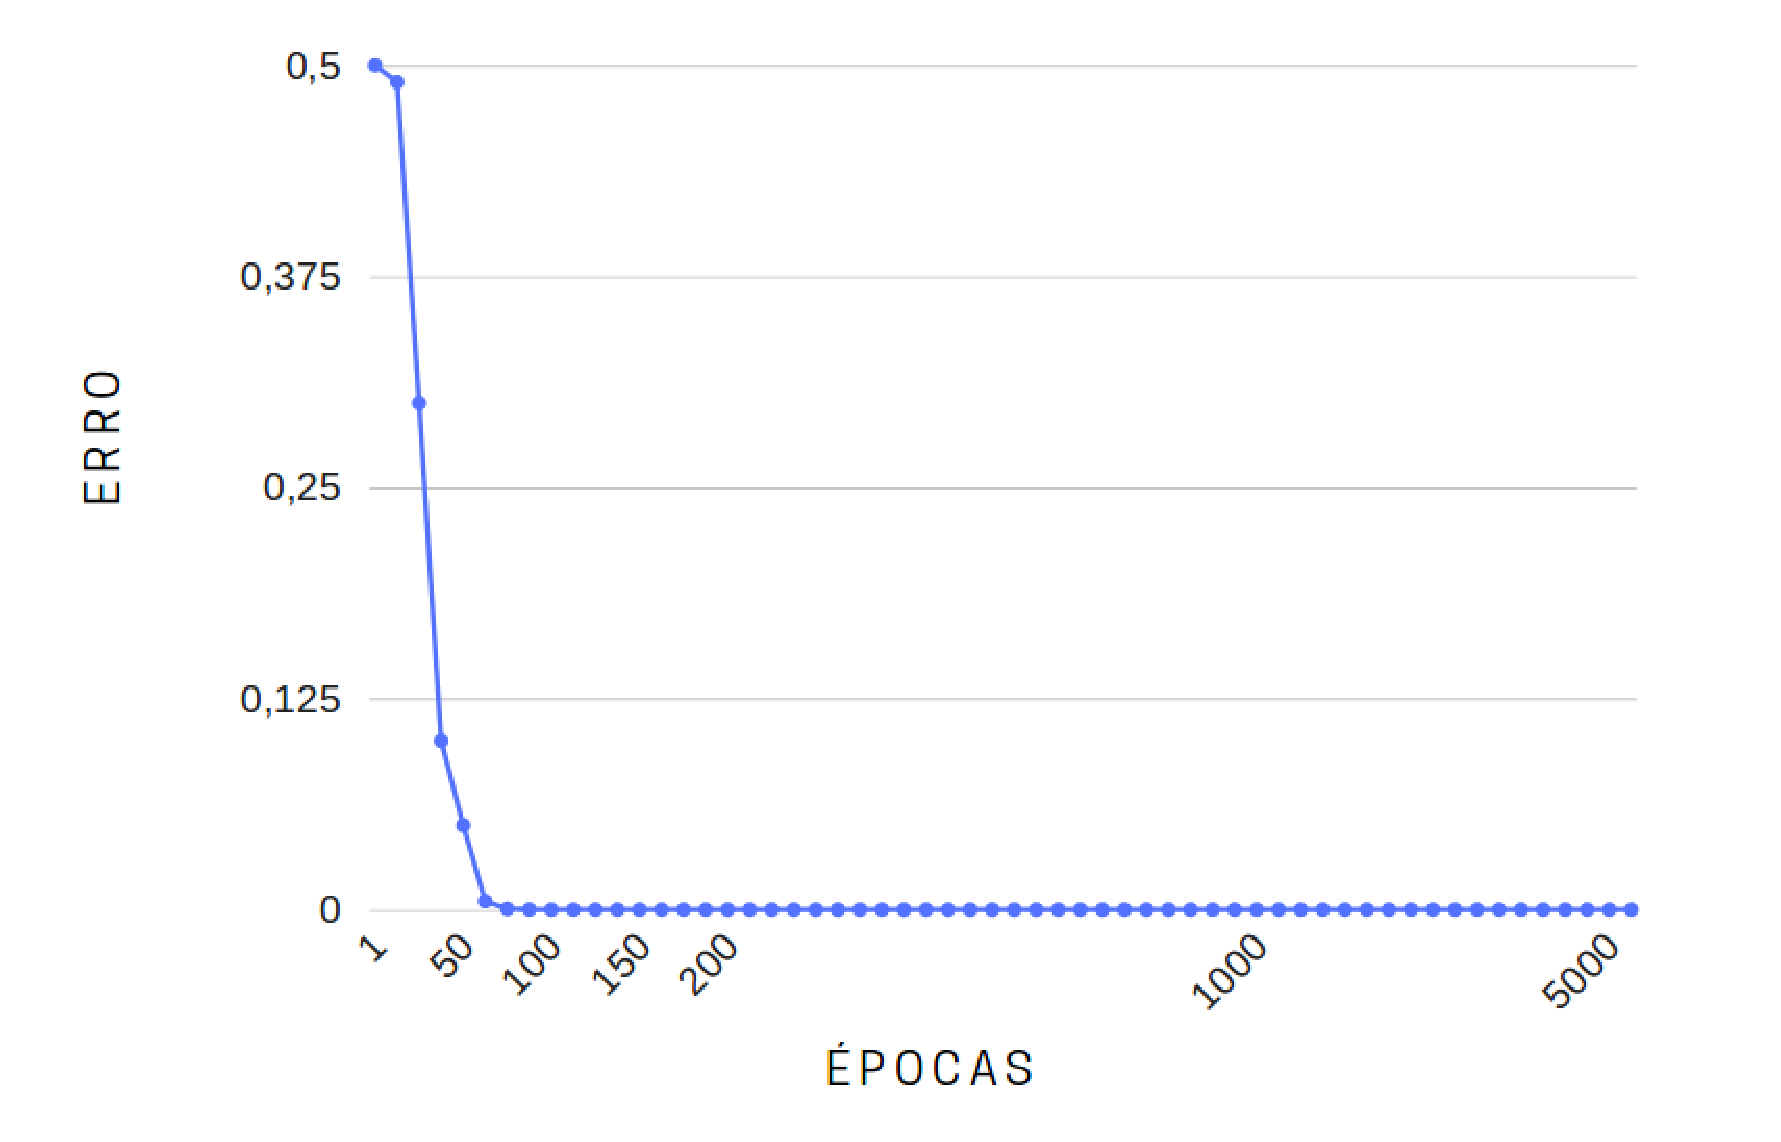
\includegraphics[keepaspectratio=true, scale=0.4]{editaveis/images/grafico_rna.eps}
%     \caption{Gráfico de Evolução da RNA}
% \end{figure} 

%  Como o processo iterativo viria a ser muito longo, foram marcados no gráfico somente os pontos onde ocorreu variação de pelo menos 1\% no valor da precisão da RNA MLP. O salto de produtividade da precisão da RNA MLP se deve à uma decisão de projeto de dividir cada uma das imagens produzidas na sessão de fotos em quadrados de 32x32 \textit{pixels}, aumentando assim a amostra de imagens geradoras de dados para treinamento da RNA, além do início do uso de \textit{bias}.


% - - - - falar sobre IA explicitamente - - - -  \\
% - - - - descrever resultados de rna com estatística - - - -  